\chapter{Data Collection}

\section{Initial Research Question and Data Collection}

The original intent of this research project was to identify differences in commit behavior between paid and volunteer contributors of open source projects. In order to classify contributors as paid or volunteer, a script was written which collected data from various public online profiles of ASF contributors active in 2015 and computed several heuristics;  the intent was to use some of this data features 
to classify individuals as paid or volunteer. 
 However, two issues made it difficult to identify the differences between the two classes:
\begin{enumerate}
	\item \label{manypaid} For a given ASF project and time period, the proportion of active contributors who are paid to work on the project can be very high, sometimes nearing 100\%.
	\item \label{novolunteers} A profile can contain certain markers that are highly correlated with paid contributors, but there are no known markers that are highly correlated with volunteer contributors.
\end{enumerate}
Issue \#\ref{manypaid} was \emph{prima facie} quite surprising---one might expect there to be a somewhat even mix of paid and volunteer contributors, but upon manually examining contributors to a couple projects, it was discovered that these projects were almost exclusively developed by employees of a few companies during the time period under observation. With such skewed samples, it became difficult to write a classifier sensitive enough to be useful.
Issue \#\ref{novolunteers} was an unforeseen limitation of using profile information to identify social group affiliation. Ultimately, there was no reliable way to differentiate between a volunteer and a paid contributor when his/her data does not reveal any obvious link between his/her contributions and his/her employer.
Since creating this classifier proved infeasible, the data was re-purposed to do a social network analysis of ASF contributions instead. In particular, the following facets of the existing dataset were useful for this purpose:
\begin{itemize}
	\item The dataset associates data from multiple accounts/profiles to one contributor, improving the reliability of finding a given contributor's employer.
	\item Since the contributor's employer was one of the data points which the algorithm used, a fair amount of employer data was already available.
\end{itemize}

\section{Data Sources}

To find the employer of a given Git committer, the script attempts to collect data from the Git account, and any associated JIRA and/or Github accounts. It also utilizes the Google Custom Search API to find links to LinkedIn profiles, which can then be inspected manually. Each set of values is stored in a separate entry in a PostgreSQL database, to maximize the amount of information available for finding a contributor's employer.
The following information is mined from Git, Github, and JIRA accounts:
\begin{itemize}
	\item Username
	\item Email address
	\item Display name
\end{itemize}
The following additional information is mined from Git accounts:
\begin{itemize}
	\item Commit count per project
\end{itemize}
The following additional information is mined from Github accounts:
\begin{itemize}
	\item Location
	\item Company name
	\item List of organizations
\end{itemize}
Furthermore, to work around the rate limit of the Github API, the script utilized a GHTorrent.org database dump as an offline cache of Github data.

\pd{Add a section here between 2.2 and 2.3, entitled "Schema of Mined Data" explaining the schema of all your data, viz., all relations,  including accountprojects}

\section{Database Schema}
Due to technical limitations in some of the external dependencies used to obtain project and contributor data, multiple different databases were required. The following subsections describe the purpose and schema of these databases.
\subsection{GHTorrent Database}
A MySQL dump of the 2016 GHTorrent database was downloaded from GHTorrent.org and installed locally. This database was used as a cache for the live Github data, which sped up the data collection process because it provided a way to avoid encountering the Github API rate limit as frequently. The relevant portion of the schema is shown in figure \ref{fig:ghtorrentSchema}
\begin{figure}
	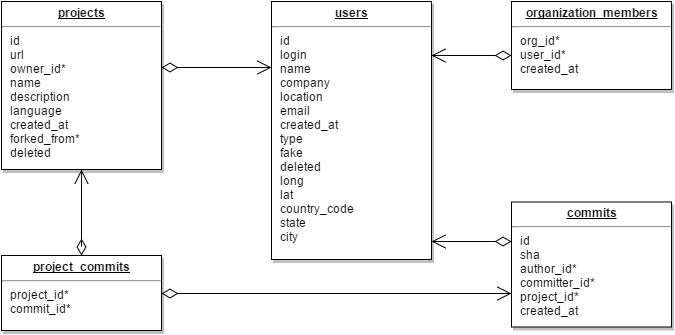
\includegraphics[width=\textwidth]{GHTorrentSchema.png}
	\centering
	\caption{The relevant tables of the GHTorrent database}
	\label{fig:ghtorrentSchema}
\end{figure}
\subsection{CVSAnalY Databases}
The cvsanaly2 tool\cite{cvsanaly} was used to parse each project's Git log data and transform it into a database that could be analyzed more quickly and conveniently. At the time of writing, cvsanaly2 only supports MySQL databases. One database was created for each project analyzed, with the name \verb|<<project_name>>_git|. The relevant portion of the schema of these databases is shown in figure \ref{fig:cvsanalySchema}.
\begin{figure}
	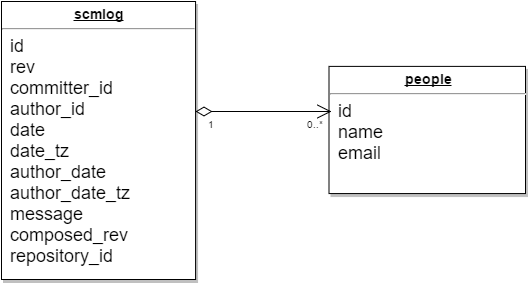
\includegraphics[scale=0.8]{cvsanalySchema.png}
	\centering
	\caption{The relevant tables of each cvsanaly2 database}
	\label{fig:cvsanalySchema}
\end{figure}
\subsection{Main Database}
The main research database contains all the data collected from Git, Github, and JIRA, and all data derived thereof. It is stored in PostgreSQL\footnote{At the time when the database was created, there was not yet a dependency on cvsanaly2 or GHTorrent, so it was created in PostgreSQL. By the point when it became clear that the dependencies required MySQL, the cost of porting the existing code to use it outweighed the benefits of using a single DBMS, so the main database remained in PostgreSQL. Since the databases were generally accessed through the SQLAlchemy ORM abstraction layer anyway, this was not too much of an inconvenience.}.

The most important tables are \textbf{contributors} and \textbf{contributoraccounts}. \textbf{contributoraccounts} stores the data for each Git, Github, and JIRA account. Each row has a foreign key to \textbf{contributors}, which allows the association of multiple accounts to a single person. The table \textbf{emailprojectcommitcount} maps an email address in the git log to the number of commits that account authored for each project. With these three tables, we derive \textbf{contributorprojectcommitcount}. The table \textbf{contributorcompanies} maps a contributor to their employer. The generation of this table is discussed in subsequent sections. Joining \textbf{contributorcompanies} and \textbf{contributorprojectcommitcount} creates \textbf{companyprojectcommitcount}, which is then used as the basis of generating the company social networks.

\section{Data Collection Constraints}
Since a contributor's employer name can only be obtained if the contributor chooses to reveal it, there will typically be some individuals for whom no employer name could be found. A further constraint is that if this information cannot be mined automatically for most people, it becomes infeasible to fill missing values in the dataset through manual inspection. After performing some case studies, it was found that this can be a significant problem for larger projects such as Apache Kafka, which have many individual committers. However, the vast majority of commits to a project typically came from a small group of the committers, whose employers could more easily be found. For this reason, the data collection was limited to only the prolific contributors of each project, defined as contributors in the minimum size set S such that the sum of the number of commits done by members of S is at least 80\% of the number of commits done to the project for the time period under observation. This also had the effect of improving the proportion of employer names mined automatically, because prolific contributors seem to be more likely to keep their Git, Github, and JIRA profile information up-to-date.
An additional constraint was that only ASF projects which met the following conditions were considered:
\begin{itemize}
	\item The project is listed in the GHTorrent.org database
	\item The project has a JIRA hosted at \ASFJIRAURL
	\item At least 20 commits were done to the project within the period under observation
\end{itemize}
These constraints resulted in the exclusion of projects which lacked sufficient data to analyze.
% TODO: do something about the overflowing table
\begin{table}
	\begin{tabular}{l|c}%
		\bfseries Organization & \bfseries Committers% specify table head
		\csvreader[head to column names]{companypeoplecount.csv}{}% use head of csv as column names
		{\\\hline\company & \personcount}% specify your coloumns here
	\end{tabular}
	\caption{Number of committers accounted for in each project}
\end{table}

\section{Data Collection Algorithm}
The script jiradb.py performs the majority of the data gathering. Its algorithm can be summarized as follows:
\begin{enumerate}
	\item Get JIRA account data for contributors to the JIRAs of the projects
	\item Get Git account and commit data for committers to the projects
	\item Get Github account data for Git accounts 
	\item Associate accounts belonging to a single person under a single contributor ID \pd{Explain how this done} 
	\item Generate a guess for the employer of each contributor \pd{Explain how this is done} 
\end{enumerate}

Each individual set of profile data is stored in a row of the \textbf{accountprojects} table of the research database. This table relates account information to an ASF project which that account contributed to. The following sections provide more details on the data collection steps.

\subsection{JIRA Data}
\pd{Use consistent typography for "JIRA"}
The jira Python package was used to query the ASF JIRA at \ASFJIRAURL. JIRA can be queried programatically by using the JIRA Query Language (JQL). The following JQL query was used to download issues for project \textbf{P} that were either created or resolved in \timeperiod:
\begin{lstlisting}
project = "P" AND created < "2016-06-01 00:00" AND (created >
 "2016-01-01 00:00" OR resolved < "2016-06-01 00:00")
\end{lstlisting}
After the issues were downloaded, each issue's metadata and history was processed to find JIRA accounts that either created or resolved the issue in \timeperiod. The profile information for each account was stored as an entry in \textbf{accountprojects}.
\subsection{Git Data}
The cvsanaly tool was used to generate databases containing structured git log data for each project. Each log database was queried to obtain the number of commits authored in \timeperiod. If it was less than 20, the project was excluded from further analysis. Otherwise, each commit author's email address was cross-referenced against the GHTorrent database to find his/her Github account(s). For each Github account found, the git account information was inserted into \textbf{accountprojects}, with the username column set to the Github account's username. Finally, if the email address had not been seen before, a row was added to table \textbf{emailprojectcommitcount} relating the address to the number of commits authored from that address to the project during \timeperiod.
\subsection{Github Data}
Whenever a new Git or JIRA account was processed, the account information was used to query the GHTorrent database to find the associated Github account. Matching against Git account information was typically more reliable than using JIRA, since Github users are encouraged to add their Git email address to their Github accounts. However, in cases where the user did not do so, sometimes they used their JIRA account's email address instead, so the accounts could be associated through that.

Technically, Github allows an email address to be associated with only one Github account, but due to inaccuracies in the GHTorrent dataset, this constraint cannot be relied upon. To mitigate this problem, a row in \textbf{accountprojects} is created for each possible Github username linked with a given email address in GHTorrent, but the only direct usage of these usernames was for identity merging purposes. In cases where actual Github profile information was needed, the usernames were validated using the Github API before use, and the first valid one was taken as the contributor's official Github username.
\subsection{Identity Merging}
Two accounts were considered to belong to the same person when at least one of the following was true:
\begin{itemize}
	\item The accounts use the same email address
	\item The accounts use the same username and service (i.e. Git or JIRA)
\end{itemize}
The only exception to these rules was that accounts which used the email address ``dev-null@apache.org'' were not paired based on the email alone, because this is a shared email address used by multiple ASF contributors. For the purpose of identity merging, Git and Github were considered to be the same service.

For each new contributor found (i.e. whenever a new account could not be associated with an existing account using the above rules), a row was added to the \textbf{contributors} table of the research database. Then, the new account information was used to query the GHTorrent database to find the associated Github account. Failing that, a similar query was performed against the live Github API. If the Github account was found, the login, company, and location values were stored in the newly created \textbf{contributors} row.

Matching Github accounts using Git account information was typically more reliable than using JIRA account information, since Github users are encouraged to add their Git email address to their Github accounts. However, in cases where the user did not do so, sometimes they used their JIRA account's email address instead, so the accounts could be associated through that.
\subsection{Employer Identification}
As described earlier, it was not always possible to pinpoint a contributor's employer with high confidence. However, it was usually possible to generate a number of guesses, 
based on the data contained in the contributor's accounts. Employer guesses were collected from account information, synthesized into a final guess for each contributor, and inspected and corrected manually.
Employer guesses were generated from the following sources:
\begin{itemize}
	\item ``Company'' field of Github profiles
	\item Domain name of email addresses
	\item LinkedIn
\end{itemize}
LinkedIn page URLs were found by using Google Custom Search API to query linkedin.com using the concatenation of each account's display name and the name of the project that account contributed to. These pages were then inspected manually to find the current employer. 